\documentclass{article}

\usepackage{tikz}
\usetikzlibrary{positioning}

\title{Interaction Diagram - Add User}
\author{Adam Hammes}

% no page number at bottom
\pagenumbering{gobble}

\begin{document}
\maketitle

\begin{center}
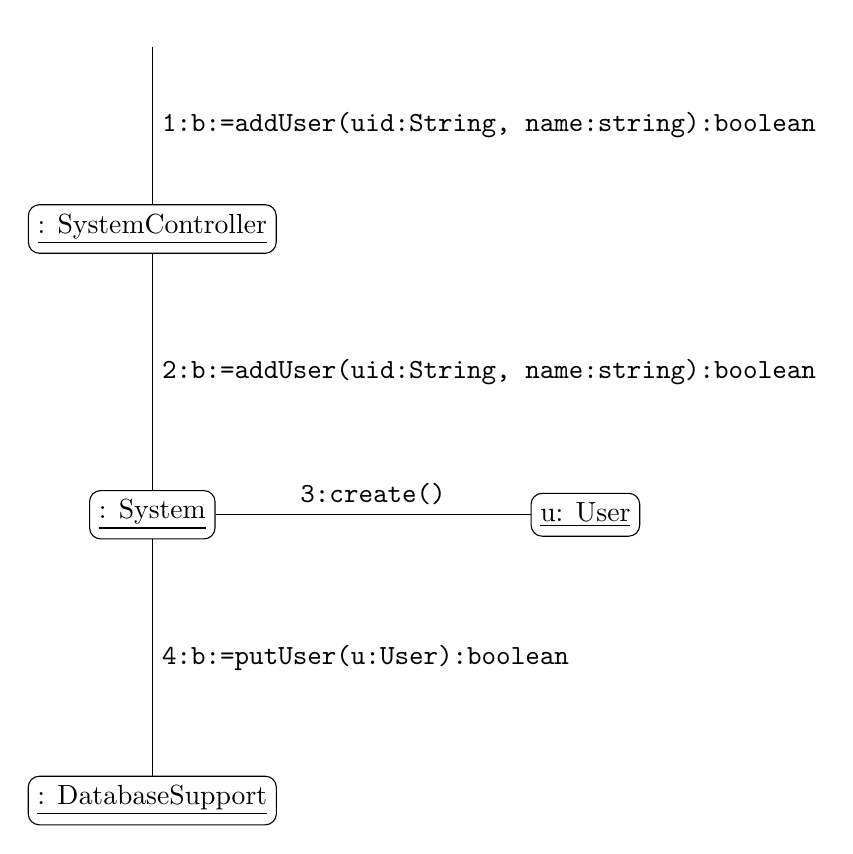
\begin{tikzpicture}[
  auto,
  block/.style = {
    rectangle,
    draw=black,
    align=center,
    rounded corners
  }
]

% Used for the arrow coming down to SystemController
\node[] (start)  {};

%     style     location                variable name    content 
\node[block, below = 2cm of start]      (controller) {\underline{: SystemController}};
\node[block, below = 3cm of controller] (system)     {\underline{: System}}; 
\node[block, right = 4cm of system]     (user)       {\underline{u: User}};
\node[block, below = 3cm of system]     (database)   {\underline{: DatabaseSupport}};

%     (start_node) -- (end_node)   node[location] {content}
\draw (start)      -- (controller) node[midway] {\texttt{1:b:=addUser(uid:String, name:string):boolean}};
\draw (controller) -- (system)     node[midway] {\texttt{2:b:=addUser(uid:String, name:string):boolean}};
\draw (system)     -- (user)       node[midway] {\texttt{3:create()}};
\draw (system)     -- (database)   node[midway] {\texttt{4:b:=putUser(u:User):boolean}};

\end{tikzpicture}
\end{center}

\end{document}
